\noindent Identity and Access Management provides protection for resources and data through rules and policies which are enforced on users via various techniques. Common ones are enforcing login passwords, assigning privileges to the users and provisioning user accounts \cite{AlmullaSameeraAbdulrahmanandYeun2010}.
Similarly, in Google Cloud, IAM grants granular access to specific resources and helps prevent access to other resources \cite{Googlecloudiam}.

Identities are essentially authenticated members. A member (Figure~\ref{fig:mem}) can be a Google Account for end users (userid@gmail.com), a service account for apps and virtual machines (12345678@cloudservices.gserviceaccount.com), a Google group (groupname@googlegroups.com), or a G Suite or cloud identity domain that can access a resource (alias@example.com). The identities of the first three member types are email addresses. The identity associated with G Suite or cloud identity domain is usually a domain name.
\begin{figure}[h]
  \centering
  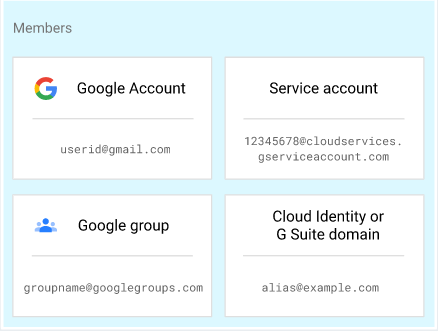
\includegraphics[width=\linewidth]{pic/mem}
  \caption {Types of Members in GCP}
  \label{fig:mem}
\end{figure}

An authorization process that grants access of resources to members can be achieved through role and policy. A role is a collection of permissions determining what operations are allowed on a resource (Figure~\ref{fig:role}). Instead of assigning permissions directly to end users, in Google Cloud, permissions are grouped into roles and then granted to authenticated members to access resources. Granting a role to a member actually grants all the permissions of that role.
\begin{figure}[!h]
  \centering
  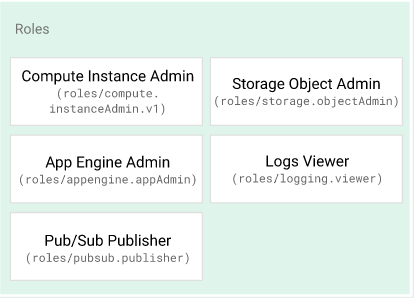
\includegraphics[width=\linewidth]{pic/role}
  \caption {GCP Predefined Role}
  \label{fig:role}
\end{figure}
A policy binds who (member) has what access (role) for which resource \cite{Googlecloudiam}. Some examples of resources are organizations, folders, projects, Compute Engine instances, and Cloud Storage buckets. The binding between members and roles is a many-to-many relationship.
Primitive, predefined, and custom roles are three types of roles supported in Google Cloud IAM \cite{googlecloudrole}. Primitive roles (renamed as Basic roles later) comprises Owner, Editor and Viewer roles, which exist prior to the introduction of IAM in GCP. For example, the account one uses to create a project will be automatically attach with Owner role. Predefined roles are finer-grained roles for a particular service or resource. Privileges can also be limited further by creating a custom role and attach permissions across services based on user selection. Unfortunately, not all permissions can be linked to Custom roles such as Datastore related permissions. 

The role based model of cloud IAM simplifies the implementation of PoLP. To illustrate this, we can take the access control of Cloud Storage as an example. In Cloud Storage, everything that must be contained in a bucket. Buckets are the basic containers that hold objects such as files, images, etc. Suppose in a project, a set of users need access to view files and file content in a public bucket. For beginners, an easy solution is to create a Google group for the users and grant Storage Admin role (roles/storage.admin) to it. However, looking through Table~\ref{table:sto-role}, which demonstrates all predefined Cloud Storage roles and corresponding permissions, it is obvious that Storage Object Viewer role would be sufficient for users to perform the same task. 
\begin{table}[t]
    \caption{IAM roles for Cloud Storage} \centering
    \begin{tabular}{|p{4.2cm}|p{4cm}|}
    \hline
    Role & Permissions\\
    \hline
    \hline
    Storage Object Creator\par(roles/storage.objectCreator) &  resourcemanager.projects.get \par resourcemanager.projects.list \par storage.objects.create \\ %% $\pm$ \\
    \hline
    Storage Object Viewer\par(roles/storage.objectViewer) & resourcemanager.projects.get\par resourcemanager.projects.list\par storage.objects.get\par storage.objects.list \\ %% $\pm$ \\
    \hline
    Storage Object Admin\par(roles/storage.objectAdmin) & resourcemanager.projects.get \par resourcemanager.projects.list\par storage.objects.*\\ %% $\pm$ \\
    \hline
    Storage HMAC Key Admin\par(roles/storage.hmacKeyAdmin) &storage.hmacKeys.*\\
    \hline
     Storage Admin\par(roles/storage.admin) &firebase.projects.get\par resourcemanager.projects.get\par resourcemanager.projects.list\par storage.buckets.*\par storage.objects.*\\
    \hline
    \end{tabular}
    \label{table:sto-role}
\end{table}
Therefore, Storage Object Viewer role is a better option (Figure~\ref{fig:sto-pre}), but still it is over-privileged. 
\begin{figure}[!h]
  \centering
  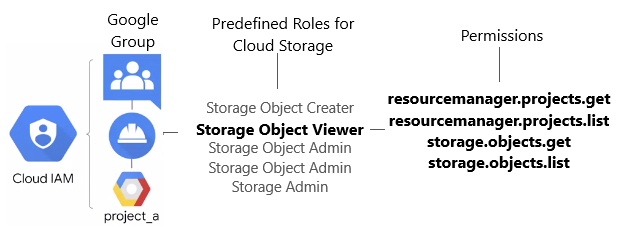
\includegraphics[width=\linewidth]{pic/sto-pre}
  \caption {Policy - Predefined Role}
   \label{fig:sto-pre}
\end{figure}
Google documentation explains that storage.objects.list and storage.objects.get are actual permissions that allow a member to list files and view file content. To follow PoLP and optimize the solution, we can create a custom role with the two least privileges attached and bind the custom role to the Google group(Figure~\ref{fig:sto-cus}).
\begin{figure}[!h]
  \centering
  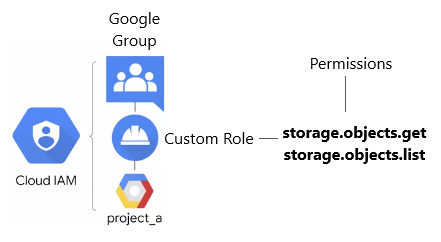
\includegraphics[width=\linewidth]{pic/sto-cus}
  \caption {Policy - Custom Role}
   \label{fig:sto-cus}
\end{figure}